\documentclass[crop,tikz,convert=pdf2svg]{standalone}

% Tikz settings optimized for causal graphs.
\usetikzlibrary{shapes,decorations,arrows,calc,arrows.meta,fit,positioning}
\tikzset{
	-Latex,auto,node distance =2 cm and 2 cm,semithick ,
	state/.style ={ellipse, draw, minimum width = 0.7 cm},
	point/.style = {circle, draw, inner sep=0.04cm,fill,node contents={}},
	bidirected/.style={Latex-Latex,dashed},
	el/.style = {inner sep=2pt, align=left, sloped}
}

\begin{document}   

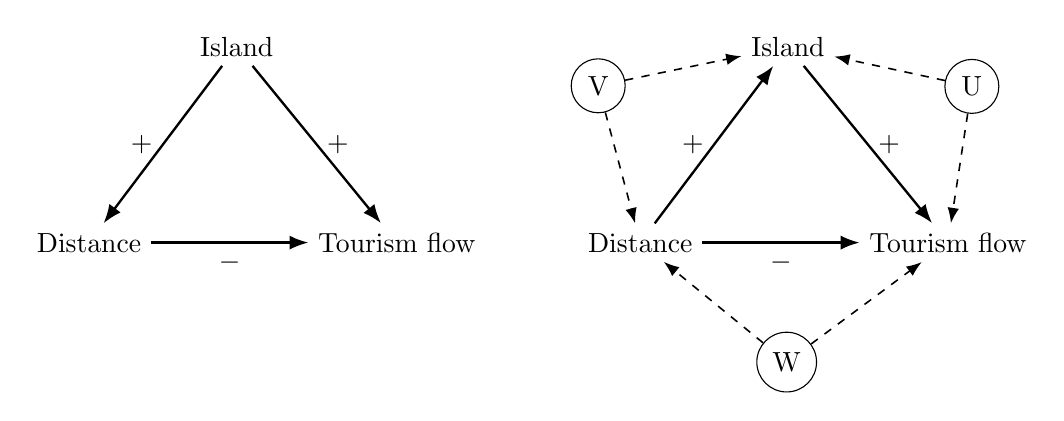
\begin{tikzpicture}

    \node (1) at (0,0) {Distance};
    \node (2) [right = of 1] {Tourism flow};
    \node (3) [above right =of 1,xshift= -1.5cm] {Island};

    \path (1) [line width=0.03cm] edge node[below] {$-$} (2);
    \path (3) [line width=0.03cm] edge node[right] {$+$} (2);
    \path (3) [line width=0.03cm] edge node[left] {$+$}  (1);
    
    \node (1) at (7,0) {Distance};
    \node (2) [right = of 1] {Tourism flow};
    \node (3) [above right =of 1,xshift=-1.5cm] {Island};
    \node[circle, draw] (4) [above right =of 3, yshift=-3cm, xshift = -0.5cm] {U};
    \node[circle, draw] (5) [above left  =of 1, yshift=-0.5cm, xshift = 2.5cm ] {V};
    \node[circle, draw] (6) [below right =of 1, yshift=1cm, xshift = -1.2cm] {W};
    
    \path (1) [line width=0.03cm] edge node[below] {$-$} (2);
    \path (3) [line width=0.03cm] edge node[right] {$+$} (2);
    \path (1) [line width=0.03cm] edge node[left] {$+$}  (3);
    \path (4) [line width=0.02cm, dashed] edge  (3);
    \path (4) [line width=0.02cm, dashed] edge  (2);
    \path (5) [line width=0.02cm, dashed] edge  (1);
    \path (5) [line width=0.02cm, dashed] edge  (3);   
    \path (6) [line width=0.02cm, dashed] edge  (1);
    \path (6) [line width=0.02cm, dashed] edge  (2);   
    
\end{tikzpicture}
\end{document}
